% \documentclass[../../Orator]{subfiles}
\documentclass[class={myRUCProject}, crop=false]{standalone}
\IfStandalone{%
    \import{../../}{customCommands}
    \import{../../}{INP-00-glossary}
    }{}
    
\begin{document}

The attempt to find an equation which can accurately describe the behavior of a chosen system is one of the most fundamental aspects of mathematics.

A model is a series of mathematical equations capable of replicating the behavior of a system. A role of these models, known as dynamic systems, is to bring light in the gaps of understanding and explain the underlying mechanisms behind some function. 
The construction of a model requires equations complex enough to accurately describe the dynamics of interest yet, preferably, simple enough so that mathematical tools exist to analyze the equations\footnotemark. 
\footnotetext{The best model of a cat is a cat. Preferably the same cat\footnotemark.-`\textit{Philosophy of Science, 1945, Arturo Rosenblueth \br*{1900-1970}}'}
There exists any number of limitations in the pursuit of this task, some inherent to the system, others inherent to our modern construction of mathematics.
\footnotetext{If man could be crossed with the cat, it would improve man, but it would deteriorate the cat.-`\textit{Mark Twain}'.}











\section{Scale of model}
 Scaling neural models is a multidimensional challenge involving trade-offs between model complexity, computational efficiency, and the ability to provide meaningful insights into neural function.
 In scaling processes the complexity of a system will often change. In the description of neuronal dynamics  from single-neuron level to network some kind of middleground in complexity will have to be reached. To describe ...
 
 What layer of information is of interest to probe?
 A description of neuronal dynamics
 As can be seen in figure \ref{fig:scale} the information that is available is different depending on what scale you are operating at.
 
 \begin{figure}[H]
    \centering
    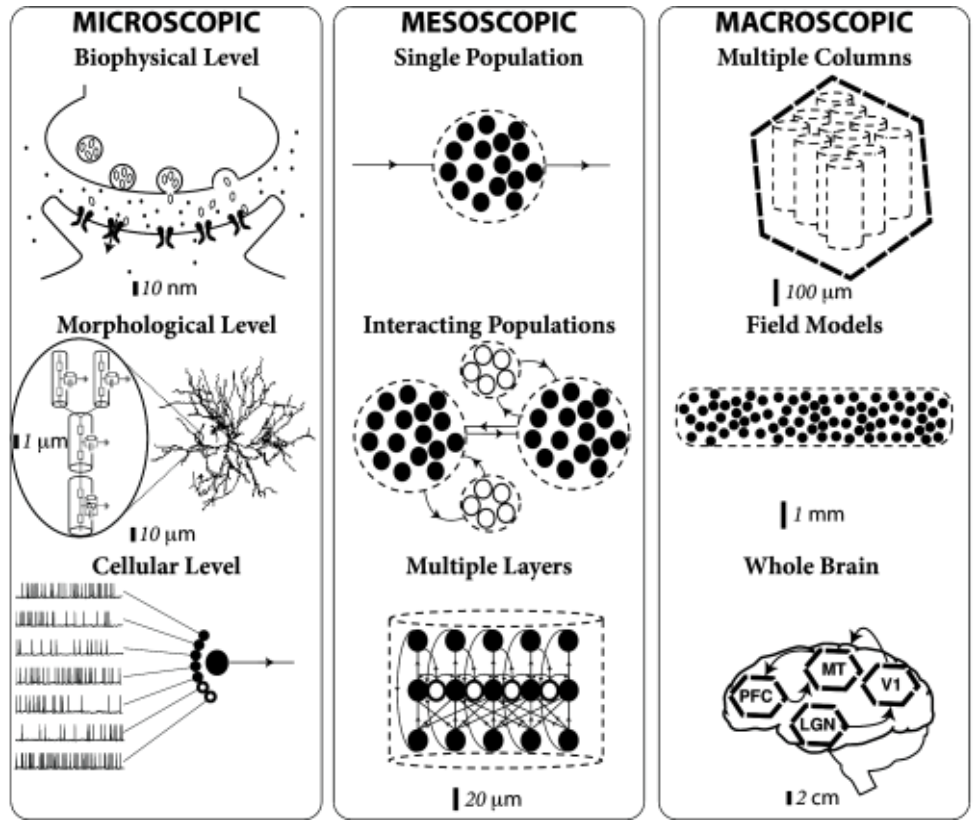
\includegraphics[width = 0.75\textwidth]{Pictures/Kenni/Level of description.png}
    \caption{Level of description, ~\cite{Burger2017}.}
    \label{fig:scale}
\end{figure}
 

\subsection{Mathematical scaling}

 
 
 figure\ref{fig:computational_properties} the 

cf. appendix\cref{fig:sum_spike_neuro} on the summery of different spiking scenarios.


For neural networks scaling up involves increasing the number of neurons interacting and to capture the realism the number of parameters will have to increase as well.






....


\begin{figure}[H]
    \centering
    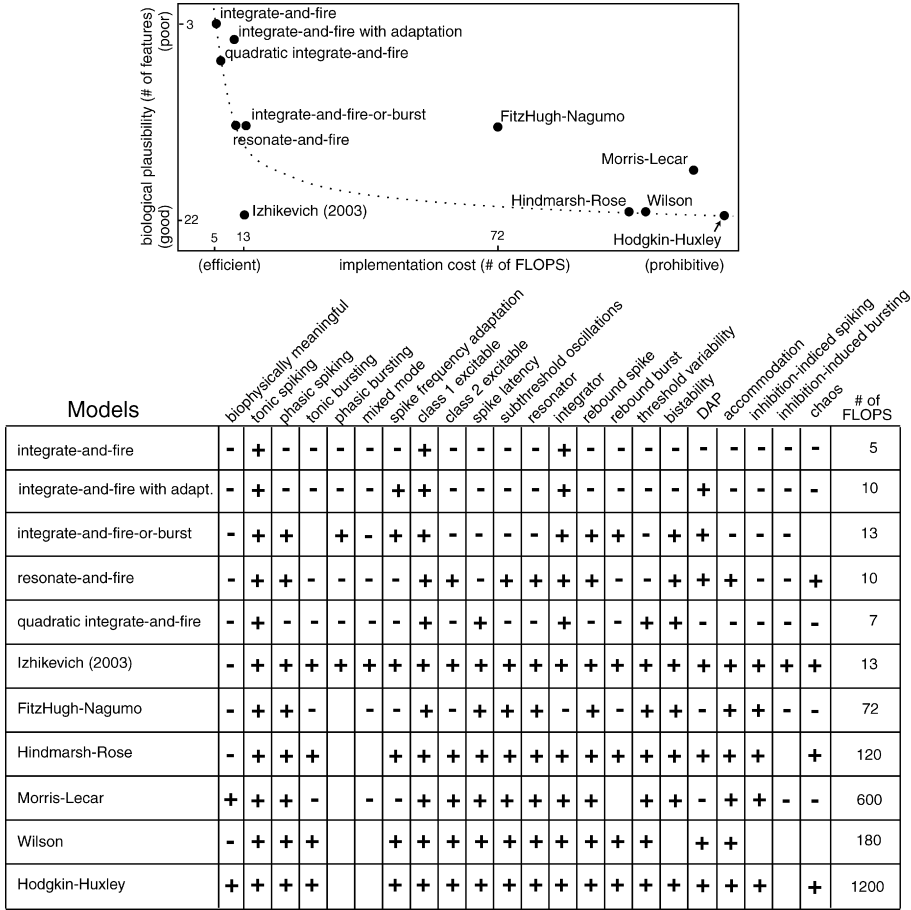
\includegraphics[width = 0.75\textwidth]{Pictures/Kenni/properties_spiking_bursting_models_all.png}
    \caption{“\# of FLOPS” is an approximate number of floating point operations (addition, multiplication, etc.) needed to simulate the model during a 1 ms time span. Each empty square indicates the property that the model should exhibit if the parameters are chosen appropriately, ~\cite{izhikevich2004model}.}
    \label{fig:computational_properties}
\end{figure}


Should be transferred to glossary section. What are:
- regimes (e.g. quiet regime)
- voltage traces
- 



\section{Dynamic System Fundamentals}
When looking at the brain in abstract form it can be seen as a multi-dimensional \gls{gls:dynSystem} governed by an independent set of system variables, such as neuronal membrane potentials, which change in time based on a set of \gls{gls:deterministic} equations with system parameters that either do not change in time (e.g. maximal \gls{gls:cond} of the ion
channels on the neuronal membrane) or whose evolution happens on a much slower time scale relative to the evolution of the system variables ~\cite{STEFANESCU2012748}.


Fundamentally, a \gls{gls:dynSystem} is a system that evolves over time.  This system is dependent on fixed rules which govern the evolution of the system. Thus a \gls{gls:dynSystem} is the opposite of a static system, which, unlike \gls{gls:dynSystem}s, does not depend on the past inputs. A simple example of a \gls{gls:dynSystem} can be that of a pendulum swinging back and forth \cite{}. 

There are different types of \gls{gls:dynSystem}s. A system can be \gls{gls:deterministic} or \gls{gls:stochastic}, \gls{gls:discrete} or \gls{gls:continuous}, \gls{gls:linear} or \gls{gls:nonlinear}, and \gls{gls:autonomous} or \gls{gls:non-autonomous} \cite{}. 

If a system is \gls{gls:deterministic}, it is possible to predict each following state given an initial state. It is also possible for a system to have an element of randomness to it. In this case, the system is said to be \gls{gls:stochastic} \cite{}. 

A \gls{gls:discrete} system is one where there is only measured a position of the integer values of time. On the other hand, is a \gls{gls:continuous} system, where the positions are measured \gls{gls:continuous}ly (ie. for every possible time) \cite{}.

A \gls{gls:linear} system is one where it is only composed of \gls{gls:linear} functions and a \gls{gls:nonlinear} system contains at least one \gls{gls:nonlinear} component \cite{}.

Lastly, there is the difference between an \gls{gls:autonomous} system, which is one where it does not depend on the independent variable \(t\) \cite{}, and a \gls{gls:non-autonomous} system, which does depend on \(t\) \cite{}.

%The 
%Some of these parameters

\begin{comment}
    \begin{split}\left[\begin{array}{ccll}
    {\displaystyle \frac{du}{dt}} &=& u\left(1-u^{2}\right)-w+I \equiv F(u,w)\\[.2cm]
    {\displaystyle \frac{dw}{dt}} &=& \varepsilon \left(u -0.5w+1\right) \equiv \varepsilon G(u,w)\, ,\\
    \end{array}\right.\end{split}
    [ref:https://neuronaldynamics-exercises.readthedocs.io/en/latest/exercises/brunel-network.html]
\end{comment}

When analysing differential equations \textit{phase space} analysis is an important concept and tool. Phase space is the space spanned by the system's variables and the trajectories it contain are those variables traversing time. When a neuron transitions from rest to firing a qualitative change in the dynamical behavior of the system will occur. A qualitative change can be associated with phenomena such as \textit{bifurcations}, \textit{phase transitions}, emergence of (new) \textit{attractors}, or shifts in stability. 

Bifurcations constitutes critical points where the stability of a system changes, leading to abrupt transitions in the system's behavior. As will be shown these transitions can provide insights into the onset of seizures and their characteristics [link to network analysis section]


Let's consider a simple two-variable system where the variables represent the activity of excitatory and inhibitory neurons. A phase plane for such a system could help visualize the dynamics.

Here's a simple set of differential equations to represent this system:
%\(P(k)  \sim  k^\gamma\)


%\begin{sysEquation}\label{eq:Power-law}
 %   P(k)  \sim  k^\gamma
%\end{sysEquation}
dxdt = alpha * (1 - x**2) - beta * y
dydt = gamma * x - delta * y

%This is a simplified version of the FitzHugh-Nagumo model, commonly used to study excitable systems. Parameters α, β, γ, and 
%δ control the behavior of the system.

\begin{figure}[H]
    \centering
    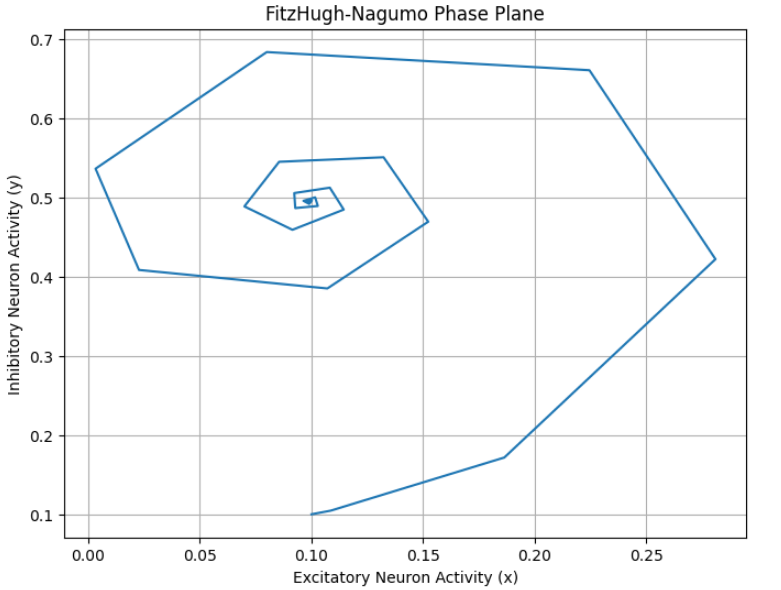
\includegraphics[width = 0.75\textwidth]{Pictures/Kenni/FitzHugh-Nagumo Phase Plane.png}
    \caption{Caption}
    \label{fig:Phase_Plane}
\end{figure}

Notes:
- Time delays can be the source of instabilities and bifurcations in \gls{gls:dynSystem}s and are frequently observed in biological systems such as neural networks.
- with qualitative change in the dynamical behavior of the system we mean 
- The bifurcation constitutes a 'dividing event' and is associated with modifications to the system parameters such as membrane capacitance and ion channel parameters etc. ~\cite{STEFANESCU2012748}.
- The reduced, two dimensional Hodgkin-Huxley model constitutes what is called a relaxation oscillator. Oscillator because solutions oscillate, there is a limit cycle. 
%Relaxation is because \v at first gradually rises, while \n falls,
“building up tension” as it were, then all of the sudden the tension is “released”
when the trajectory shoots over from the left branch of the v-nullcline to its right
branch. See example 


Bifurcations are critical points where the stability of a system changes, leading to abrupt transitions in the system's behavior. These transitions can provide insights into the onset of seizures and their characteristics.
Identifying bifurcation points in neural systems helps to understand the mechanisms underlying the transition from normal brain activity to a seizure state.

\subsubsection{Dimensionality reduction}
A neuron model, such as the \gls{hh} model, uses a system of four differential equations
to simulate a complex network this can quickly amount to an insurmountable task with contemporary computer technology...
% perhaps a note or two about what is actually needed in terms of computational operations and why a reduction in complexity is relevant??

% A Two-Dimensional Reduction of the Classical Hodgkin-Huxley Model --> SEE "An Introduction to Modeling Neuron Dynamics", (978-3-319-51171-9), page 73 in our litterature folder.





\subsection*{Modeling Neuronal Networks}
A complex system can be described by a network or a graph with complex topology, whose nodes are the elements of the system and whose edges represent the interactions among them. `One significant recent discovery in the field of complex networks is the observation that a number of large-scale and complex networks are scale-free, that is, their connectivity distributions have the
power-law form'~\cite{wang2002synchronization}.

% ...

Self-organized criticality has been proposed as a framework to understand various phenomena in nature ranging from earthquakes, forest fires to neuronal activity in the brain.
Avalanche Dynamics: In self-organized critical systems, events or disturbances can lead to cascading effects, causing a series of interconnected events or "avalanches." The size distribution of these avalanches often follows a power-law distribution ~\cite{beggs2004neuronal, plenz2007organizing}.

% ...

The power-law form in connectivity distributions refers to a specific mathematical relationship that characterizes the distribution of connections or links among elements in a network. In a power-law distribution, the probability of a node having k connections (degree) is proportional to k raised to the power of a negative exponent.

Mathematically, the power-law distribution is often expressed as:
\(P(k)  \sim  k^\gamma\)
\begin{equation}\label{eq:Power-law}
    P(k)  \sim  k^\gamma
\end{equation}

$P(k)$ is the probability that a node has $k$ connections.
$\gamma$ is the exponent characterizing the power-law distribution.


from the article : "FitzHugh-Nagumo oscillators on complex networks mimic epileptic-seizure-related synchronization phenomena":

% We study patterns of partial synchronization in a network of FitzHugh-Nagumo oscillators with empirical structural connectivity measured in human subjects. We report the spontaneous occurrence of synchronization phenomena that closely resemble the ones seen during epileptic seizures in humans. In order to obtain deeper insights into the interplay between dynamics and network topology, we perform long-term simulations of oscillatory dynamics on different
% paradigmatic network structures: random networks, regular nonlocally coupled ring networks, ring networks with fractal connectivities, and small-world networks with various rewiring probability. Among these networks, a smallworld network with intermediate rewiring probability best mimics the findings achieved with the simulations using the empirical structural connectivity. For the other network topologies, either no spontaneously occurring epileptic-seizurerelated synchronization phenomena can be observed in the simulated dynamics, or the overall degree of synchronization
%remains high throughout the simulation. This indicates that a topology with some balance between regularity and randomness favors the self-initiation and self-termination of episodes of seizure-like strong synchronization.

Notes:
- a smallworld network
- 
...



When analysing seizures, bifurcation points helps to understand the mechanisms underlying the transition from normal brain activity to a seizure state. The change in parameter can be factors like synaptic strength, excitability of neurons, or network connectivity 
~\cite{gerstner2014neuronal}. 





    
\subsubsection{Network connectivity and topology}


Modeling brain processes can be advantages because of the difficulties  performing certain experiments and it is therefore possible to simulate certain scenarios without the need of conducting large scale exploratory experiments. Aspects like ethical barriers...

The practical barriers to simulating brain processes are to do with the modeling framework of the particular question of interest together with the computational resources needed to run complex simulations. Fortunately Moore's Law is still holding and with the emergence of AI the modeling framework have been propelled foreword. Large-scale brain simulation projects, like the Human Brain Project\footnote{\url{https://www.humanbrainproject.eu/en/brain-simulation/}}, leverage AI and high-performance computing to simulate the behavior of billions of neurons and their connections.

\end{document}


\section{Building up to Hodgkin-Huxley}

The \gls{hh} Model of Neuron Action Potential is regarded as being a part of the great achievements of 20th-century biophysics. Receiving the Nobel Prize in Physiology or Medicine for what is inarguably an incredible feat of human ingenuity. However, the authors of this paper are students, and therefore such a sophisticated model might be beyond the direct reach of abilities within the given timeframe. 
As such, the exploration begins by investigating simplified \gls{hh} derived models to see what insights can be built.
%
These models are only going to be presented for now, and discussion regarding their details are to be saved for \Cref{ch:modelDis}.

\subsection{FitzHugh-Nagumo}
``The models in this category are highly simplified toy models that qualitatively describe the membrane voltage as a function of input. They are mainly used for didactic reasons in teaching but are not considered valid neuron models for large-scale simulations or data fitting''.\footnote{Wikipedia} 
%\subsubsection{Didactic toy model}
\begin{sysEquation}[FitNagSys]
    \ode{V} &= V - \frac{V^3}{3} - w + I_{ext} \\ 
    \tau\ode{w} &= V - a - b\,w 
\end{sysEquation}

\subsection{Chay}
In 1985, T.R. Chay proposed a model of three-dimensional \gls{gls:nonlinear} differential equations based on the \gls{hh} model to study chaotic behavior and show ionic events in excitable membranes. 
\begin{sysEquation}[ChaySys]
    \ode{V} &= g_\rmm{I}  m^3_\infty h_\infty \br{V_\rmm{I} - V} + g_\rmm{K, V} n^4 \br{V_\rmm{K} - V} + g_\rmm{K, C}  \frac{C}{1+C}\br{V_\rmm{K} - V} + g_\rmm{L} \br{\unit{\V\membrane} - V_\rmm{L}} \\ 
    \ode{n} &= \frac{n_\infty - n}{\tau_n} \\
    \ode{C} &= \rho \, \sbr{m^3_\infty h_\infty \br{V_c - V} - k_C C}
\end{sysEquation}

where \textit{V}, \textit{n}, and \textit{C} are membrane potential, probability of the voltage-sensitive \gls{K} channel, and intracellular concentration of \gls{Ca} ions, respectively. The Chay model parameters are adopted from \textit{`paper'} and collected in Table

The \(m_\infty\), \(h_\infty\), and \(n_\infty\) are calculated by \(y_\infty = \alpha_y / \br{\alpha_y + \beta_y} \) formula, and the explicit expressions for 
\(\alpha_m, \beta_m, \alpha_h, \beta_h, \alpha_n, \beta_n\), and \(\tau_n\) are given by:
\begin{align*}
    \alpha_m &= 0.1 \frac{ 25 + V }{1 - \exp{-0.1 \, V - 2}}, &
    \alpha_h &=  0.07 \exp{-0.05\,V -2.5}, &
    \alpha_n &= 0.01 \, \frac{ 20 + V }{ 1 + \exp{-0.1 \, V - 2}} \\
    \beta_m  &= 4 \exp{-\br{\frac{ V + 50 }{ 18 } } }, &
    \beta_h  &= \frac{ 1 }{ 1 + \exp{-0.1 \, V - 2}}, &
    \beta_n  &= 0.125 \exp{- \frac{V + 30}{80}}, \\
    \tau_n &= \frac{1}{ r_n \, \br{\alpha_n + \beta_n} }
\end{align*}



\subsection{Hodgkin-Huxley}\label{sec:HHMeth}

The \gls{hh} model of Action Potential is a system of \gls{gls:nonlinear} differentiable equations with four state variables with respect to time, \(\unit{\V\membrane}\br{t}, \ n\br{t}, \ m\br{t}, \ h\br{t}\)~\cite{HodHux1952}. The model is built from approximating the characteristics of excitable cells, such as neurons, to a circuit-like construct \cref{fig:MembraneCircut}. 

Through long term experimentation, the duo of Hodgkin and Huxley divined a model built from the observations of smooth current change as a function of pores (or channels) that were either open or closed. By using a statistical approach, H\&H generated predictions for the probability of channels being open or closed at a given time in the process~\cite{HodHux1939}. H\&H presented the model as a set of four \glspl{ode} with respect to time.
\begin{sysEquation}[HodHuxSys]
    C_m \ode{\unit{\V\membrane}} &= I_m - \br{\bar{g}_\rmm{K} n^4 \br{\unit{\V\membrane} - V_\rmm{K}} + \bar{g}_\rmm{Na} m^3 h \br{\unit{\V\membrane} - V_\rmm{Na}}  + \bar{g}_\rmm{L} \br{\unit{\V\membrane} - V_\rmm{L}}} \\
    \ode{n} &= \alpha_n \br{\unit{\V\membrane}} \br{1-n} - \beta_n \br{\unit{\V\membrane}} n \\
    \ode{m} &= \alpha_m \br{\unit{\V\membrane}} \br{1-m} - \beta_m \br{\unit{\V\membrane}} m \\
    \ode{h} &= \alpha_h \br{\unit{\V\membrane}} \br{1-h} - \beta_h \br{\unit{\V\membrane}} h 
\end{sysEquation}

The `gating' variables \(m\) and \(h\), part \(n\) describe the time dependent kinetics of the voltage
The ion channel activation/inactivation\footnotemark~probabilities, denoted by \(\alpha_p, \, \beta_p : \, \br{n,m,h} \in p\), are defined such that:
\begin{align}
    \alpha_p\br{\unit{\V\membrane}} &= p_\infty \br{\unit{\V\membrane}} / \tau_p \\
    \beta_p\br{\unit{\V\membrane}}  &= \br{1 - p_\infty \br{\unit{\V\membrane}}} / \tau_p 
\end{align}
\begin{minipage}[c]{.5\textwidth}
    With \(p_\infty\) and its inverse \(1-p_\infty\) being the steady state values for activation and inactivation respectively~\cite{HodHux1952}. 
    In the original paper by Hodgkin and Huxley, the relationships of \(\alpha_p, \text{ and }\, \beta_p\) were defined as:
    \vfill
    \begin{align*}
    n &\implies \left\{
    \begin{aligned}
        \alpha_n \br{\unit{\V\membrane}} &= 0.01 \, \cfrac{ 10 - V }{ \exp{ 10 - V } - 1} \\
        \beta_n \br{\unit{\V\membrane}}  &= 0.125 \, \exp{-\cfrac{V}{80}} 
    \end{aligned} \right.
    \end{align*}
    Where \(V = V_\rmm{rest} - \unit{\V\membrane}\) represents the polarization in \unit{\milli\volt}
\end{minipage}
\hfill
\begin{minipage}[c]{.45\textwidth}
    \begin{align*}
    m &\implies \left\{
    \begin{aligned}
        \alpha_m \br{\unit{\V\membrane}} &= 0.1 \cfrac{ 25 - V }{\exp{\cfrac{25-V}{10}} - 1} \\
        \beta_m \br{\unit{\V\membrane}}  &= 4 \, \exp{-\cfrac{V}{18}} 
    \end{aligned} \right. \\
    h &\implies \left\{
    \begin{aligned}
        \alpha_h \br{\unit{\V\membrane}} &=  0.07 \, \exp{-\cfrac{V}{20}} \\
        \beta_h \br{\unit{\V\membrane}}  &= { \cfrac{1}{\exp{\cfrac{30 - V}{10}} + 1}}
    \end{aligned} \right.
    \end{align*}
\end{minipage}


\footnotetext{\underline{a}ctivation gives \(\alpha\), \underline{b}nactivation gives \(\beta\), really these are the obvious choices}



